%\documentclass[a4paper]{article}
\usepackage[utf8]{inputenc}
\usepackage[spanish, es-tabla, es-noshorthands]{babel}
\usepackage[table,xcdraw]{xcolor}
\usepackage[a4paper, footnotesep = 1cm, width=20cm, top=2.5cm, height=25cm, textwidth=18cm, textheight=25cm]{geometry}
%\geometry{showframe}

\usepackage{tikz}
\usepackage{amsmath}
\usepackage{amsfonts}
\usepackage{amssymb}
\usepackage{float}
\usepackage{graphicx}
\usepackage{caption}
\usepackage{subcaption}
\usepackage{multicol}
\usepackage{multirow}
\setlength{\doublerulesep}{\arrayrulewidth}
\usepackage{booktabs}

\usepackage{hyperref}
\hypersetup{
    colorlinks=true,
    linkcolor=blue,
    filecolor=magenta,      
    urlcolor=blue,
    citecolor=blue,    
}

\newcommand{\quotes}[1]{``#1''}
\usepackage{array}
\newcolumntype{C}[1]{>{\centering\let\newline\\\arraybackslash\hspace{0pt}}m{#1}}
\usepackage[american]{circuitikz}
\usetikzlibrary{calc}
\usepackage{fancyhdr}
\usepackage{units} 

\graphicspath{{../Ejercicio-1/}{../Ejercicio-2/}}

\pagestyle{fancy}
\fancyhf{}
\lhead{22.67 - Señales Aleatorias}
\rhead{Lambertucci, Londero B., Moriconi, Musich, Tolaba}
\rfoot{Página \thepage}
%
%\begin{document}

\subsection{Introducción}

Se analiza una secuencia $X(n)$, estimando y calculando parámetros de interés, como lo son la autocorrelación, los coeficientes de correlación parcial y la densidad espectral de potencia.

\subsection{Autocorrelación} 

Se estiman la autocorrelación mediante el uso de los primeros $128$ elementos de la secuencia brindada. Para ello, se vale los estimadores polarizados ($R_{p}$) y no polarizados ($R_{np}$) de dicho parámetro. Estas funciones son las empleadas para estimar otras funciones mediante información digitalizada.
\begin{equation}
\begin{gathered}
	R_{p}(k) = \frac{1}{N} \sum_{i=0}^{N-k-1} X(i)X(i+k)	\\
	R_{np}(k) = \frac{1}{N-k} \sum_{i=0}^{N-k-1} X(i)X(i+k)
\end{gathered}
\end{equation}
En ellas se observan los parámetros $N$, es decir, el largo de $X(n)$, y $k$, variable que puede tomar los valores $0, 1, ... \ , 127$. Mediante el uso de estos estimadores, se normaliza para poder obtener los coeficientes de autocorrelación $r_{XXp}$ y $r_{XXnp}$. 

\begin{figure}[H]
\centering
	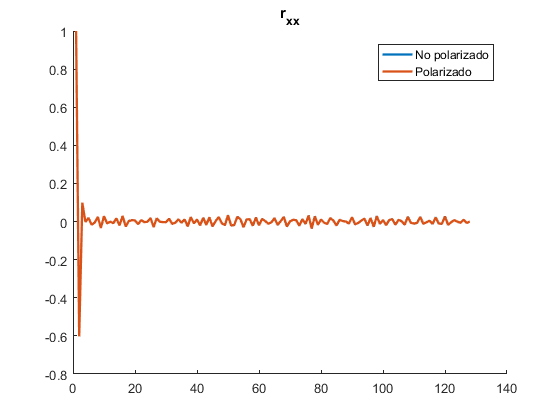
\includegraphics[width=0.8\textwidth, trim = {0 0 0 0.7cm},clip]{./ImagenesEjercicio2/rxx.png}
	\caption{Grafica de los coeficientes de autocorrelación total estimados.}
	\label{fig:rxx}
\end{figure}

Se puede observar en la Figura (\ref{fig:rxx}) como ambas curvas se encuentran solapadas, haciendo que sea prácticamente imposible distinguirlas.
Esto se debe a que existe una relación entre cada estimador, siendo esta
\begin{equation*}
\begin{gathered}
	R_{p}(k) = \frac{N - k}{N} R_{np}(k)
\end{gathered}
\end{equation*}

Ya que, para el caso del vector analizado, se da la condición de que $N = 4096$ y además $N >> k_{max} = 127$, siendo entonces
\begin{equation*}
\begin{gathered}
	R_{p}(k) \approx R_{np}(k)
\end{gathered}
\end{equation*}

\subsection{Coeficientes de correlación parcial}

Con los datos ya extraídos y mediante la resolución de la ecuación de Yule-Walker, fue posible obtener los coeficientes deseados. Esto se realizó con los coeficientes totales obtenidos a través de las estimaciones polarizada y no polarizada.
\begin{figure}[H]
\centering
	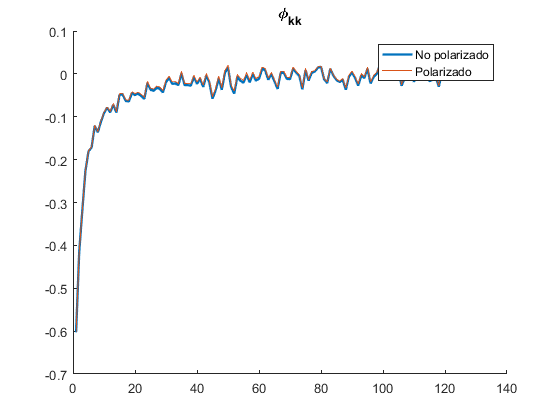
\includegraphics[width=0.7\textwidth, trim = {0 0 0 0.7cm},clip]{./ImagenesEjercicio2/phikk.png}
	\caption{Grafica de los coeficientes de autocorrelación parcial obtenidos.}
	\label{fig:phikk}
\end{figure}

En la Figura (\ref{fig:phikk}) se obtuvo nuevamente una diferencia entre ambas curvas, la cual no es significativa.

\subsection{Modelo del proceso}
\label{subsec:modelo}

Se procede a determinar que tipo de modelo utilizar para el proceso analizado. Observando la Figura (\ref{fig:rxx}), se denota que $r_{XX}(1)$ y $r_{XX}(2)$ son valores distintos de 0 ($-0,603$ y $0,099$ para ambas aproximaciones), mientras que los valores siguientes, si bien no son exactamente 0, son todos menores en modulo a $0,03$, lo que permite aproximarlos a 0. Además, observando la Figura (\ref{fig:phikk}), se puede afirmar que los $\phi_{kk}$ presentan un comportamiento exponencial. Es por ello que se determina que el proceso es un \textbf{MA(2)} (\textbf{ARMA(0,2)}).

Para el calculo de los $\theta$, se utilizaron las ecuaciones
\begin{equation}
	r_{XX}(1) = \frac{R_{XX}(1)}{\sigma_X^2} = \frac{\theta_{2,1} + \theta_{2,1} \theta_{2,2}}{1 +\theta_{2,1}^2 + \theta_{2,2}^2}
\end{equation}
\begin{equation}
	r_{XX}(2) = \frac{\theta_{2,2}}{1 +\theta_{2,1}^2 + \theta_{2,2}^2}
\end{equation}

Resolviendo dicho sistema, se obtienen los siguientes valores:
\begin{equation}
\begin{gathered}
	\theta_{2,1} = -1,280	\\
	\theta_{2,2} = 0,268	
\end{gathered}
\end{equation}

Con lo ya dicho, se procede a estimar los parámetros del proceso y compararlos con los ya obtenidos.

\begin{figure}[H]
\centering
	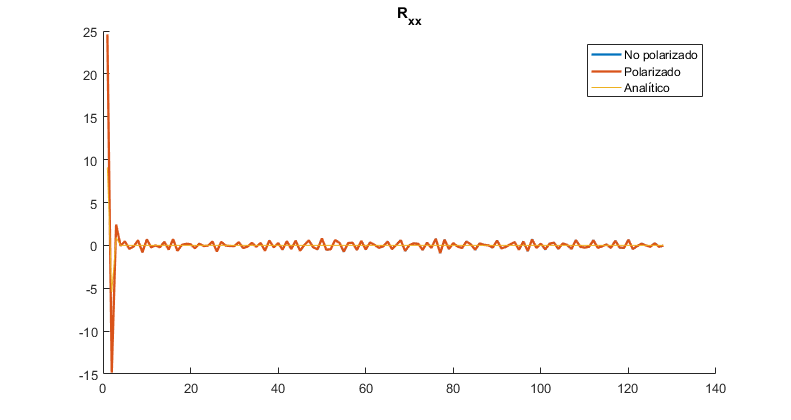
\includegraphics[width=0.8\textwidth, trim = {0 0 0 0.7cm},clip]{./ImagenesEjercicio2/Rxxcalc.png}
	\caption{Comparación de los coeficientes de autocorrelación.}
	\label{fig:Rxxcalc}
\end{figure}
\begin{figure}[H]
\centering
	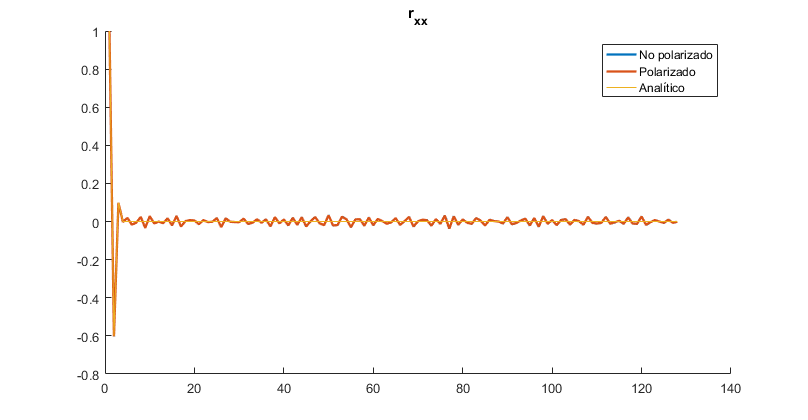
\includegraphics[width=0.8\textwidth, trim = {0 0 0 0.7cm},clip]{./ImagenesEjercicio2/rrxxcalc.png}
	\caption{Comparación de los coeficientes de autocorrelación normalizados.}
	\label{fig:rrxxcalc2}
\end{figure}

\subsection{Densidad espectral de potencia}

A continuación, se estima la la densidad espectral de potencia del vector $X(n)$. Para ello, se emplean dos técnicas distintas. La primera consiste en el uso de la transformada de Fourier de la estimación realizada de las funciones de autocorrelación.
\begin{figure}[H]
\centering
	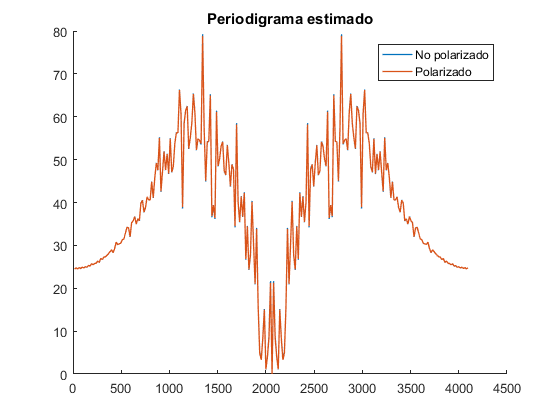
\includegraphics[width=0.8\textwidth, trim = {0 0 0 0.735cm},clip]{./ImagenesEjercicio2/period-est.png}
	\caption{Periodigramas obtenidos a partir de las estimaciones de $R_{XX}$.}
	\label{fig:period-est}
\end{figure}

%A continuación se comparan los estimaciones obtenidas previamente con la curva obtenida a partir de lo calculado en la Subsección (\ref{subsec:modelo}).
%\begin{figure}[H]
%\centering
%	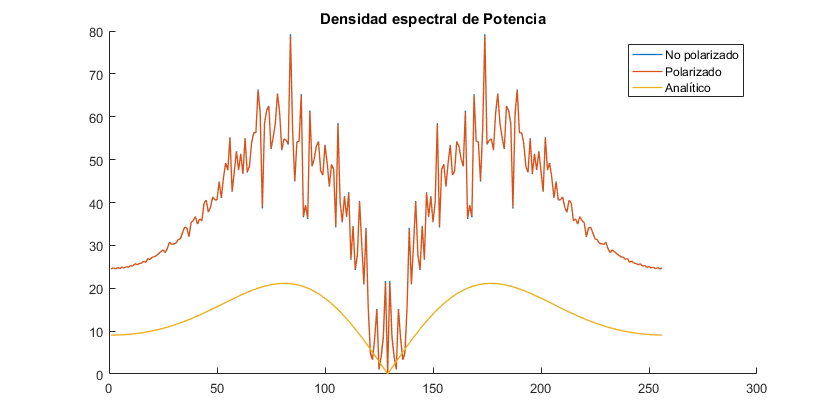
\includegraphics[width=0.7\textwidth, trim = {0 0 0 0.725cm},clip]{./ImagenesEjercicio2/densidadPot.png}
%	\caption{Comparación de periodigramas.}
%	\label{fig:densidadPot}
%\end{figure}

Como era de esperarse, la diferencia entre el gráfico obtenido a través de la estimación polarizada no difiere tanto de la no polarizada.

La segunda técnica consta de la promediación de periodigramas. Para esto se partió el vector original en 16 grupos de 256 elementos, en cada grupo se calculó los primeros 128 valores de la autocorrelacion con el estimador no polarizado, luego a cada vector se le calcula la densidad espectral de potencia y finalmente se las promedia.\footnote{Se utilizó la formula 9.24 del libro}
\begin{figure}[H]
\centering
	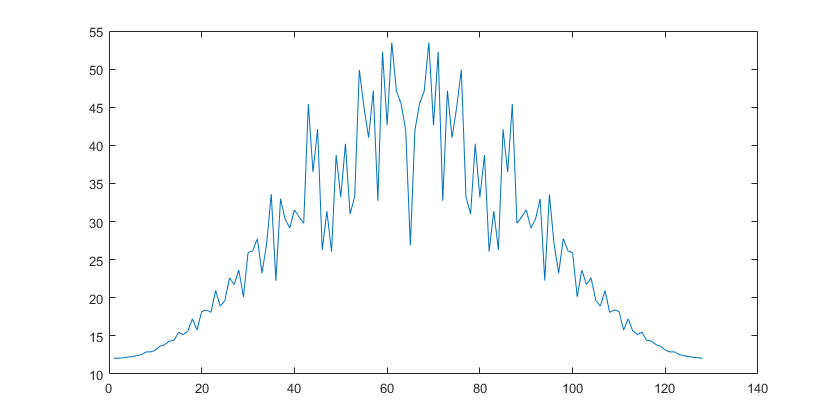
\includegraphics[width=0.8\textwidth, trim = {0 0 0 0.725cm},clip]{./ImagenesEjercicio2/period-calc.png}
	\caption{Estimación de la densidad espectral de potencia mediante el uso de promediación de periodigramas.}
	\label{fig:fft-calc}
\end{figure}



Finalmente, a modo comparativo, se ilustran las estimaciones obtenidas superpuestas:
\begin{figure}[H]
\centering
	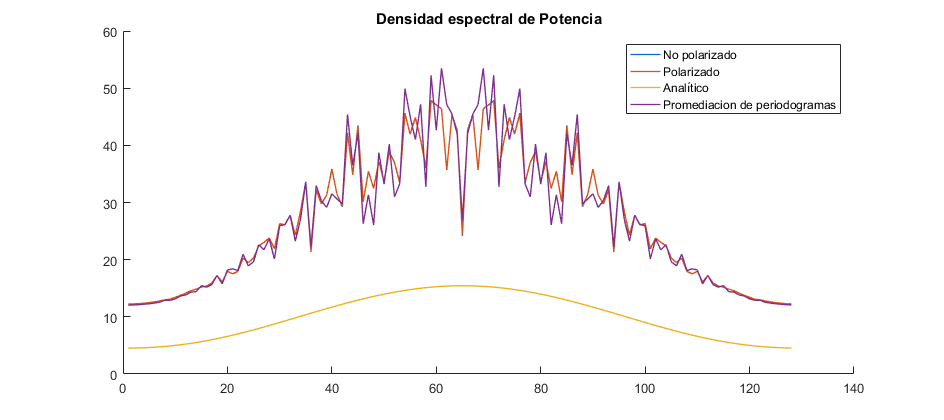
\includegraphics[width=0.8\textwidth, trim = {0 0 0 0.725cm},clip]{./ImagenesEjercicio2/fft2.png}
	\caption{Estimaciones de potencia.}
	\label{fig:fft2}
\end{figure}
Se puede apreciar que son muy similares tanto la promediación de periodogramas con la transformada de la estimación de la función de autocorrelación.
%\end{document}